\documentclass[landscape,footrule]{foils}
\usepackage[lecture-serie]{foiltex-extra}
\usepackage{crysymb}
\usepackage{graphics}
\usepackage[pdftex]{graphicx} 




\newcommand{\lecture}{Graphical models}
\newcommand{\lserie}{LTAT.02.004 Machine Learning II}
\newcommand{\ldate}{March 13, 2019}
\newcommand{\lauthor}{Sven Laur}
\newcommand{\linst}{University of Tartu}
\graphicspath{{./illustrations/}}


\newcommand{\leqm}{\ \leq_m}

\newcommand{\EVPOS}{\textcolor{red}{\mathsf{evidence}^+}}
\newcommand{\EVNEG}{\textcolor{blue}{\mathsf{evidence}^-}}

\newcommand{\bigvskip}{\vskip 2em}
\newcommand{\lastline}{\vspace*{-2ex}}
\newcommand{\spreadappart}{\vspace*{\fill}}

\DeclareMathOperator{\supp}{supp}
\DeclareMathOperator{\conf}{conf}
\DeclareMathOperator{\precision}{precision}
\DeclareMathOperator{\recall}{recall}


\begin{document}
\titlefoil


\foilhead[-1cm]{Discrete random variables}

\enlargethispage{0.9cm}
\begin{triangles}
\item A \emph{random variable} $X$ with possible \emph{outcomes} $x\in\supp(X)$
\item Compact notation for probabilities \vspace*{-1ex}
\begin{align*}
\pr{x_1}&:=\pr{\xi\gets X_1: \xi=x_1}\\
\pr{x_1\wedge x_2}&:=\pr{\xi_1\gets X_1,\xi_2\gets X_2 : \xi_1=x_1\wedge \xi_2=x_2}
\end{align*}\vspace*{-4ex}
\item Bayes formula \vspace*{-2ex}
\begin{align*}
\pr{a|b}=\frac{\pr{a\wedge b}}{\pr{b}}=\frac{\pr{b|a}\pr{a}}{\pr{b}}
\end{align*}\vspace*{-4ex}
\item Independence of random variables $X_1\ldots X_m\perp Y_1,\ldots Y_n$: \vspace*{-1ex}
\begin{align*}
 \pr{x_1\wedge\ldots\wedge x_m\wedge y_1\wedge\ldots\wedge y_n}=\pr{x_1\wedge\ldots\wedge x_m}\cdot\pr{y_1\wedge\ldots\wedge y_n}
\end{align*}\vspace*{-4ex}
\item Marginalisation over variables $Y_1,\ldots, Y_n$: \vspace*{-1ex}
\begin{align*}
 \pr{x_1\wedge\ldots\wedge x_m}=\sum_{y_1,\ldots,y_n}\pr{x_1\wedge\ldots\wedge x_m \wedge y_1\wedge\ldots\wedge y_n}
\end{align*} 
\end{triangles}

\middlefoil{Common models}

\foilhead[-1cm]{Markov chain}
\illustration[scale=1.5]{markov-chain}

\textbf{Definition.}
Let $X_1, X_2,\ldots$ be correlated random variables such that the probability of the observation $x_{i+1}$ depends only on the observation $x_{i}$.
Then the entire process is known as Markov chain.

\vspace*{1cm}

\textbf{Parametrisation.}
Markov chain is determined by specifying 

\begin{triangles}
\item state spaces $\SSS_1\ldots,\SSS_n$
\item initial probabilities $\pr{x_1}$
\item state transition probabilities $\pr{x_{i+1}|x_{i}}$
\end{triangles}

\foilhead[-1cm]{What questions can we ask?}

\textbf{Sampling:} What are typical outcomes of the chain?\\
$\triangleright$ Synthesis of time-series, textures, sounds, games movements. 
\vspace*{1.5ex} 

\textbf{Stationary distribution:} What happens if we run the chain infinitely long?\\
$\triangleright$ Getting samples from an unnormalised posterior, optimisation tasks. 
\vspace*{1.5ex}  

\textbf{Likelihood estimation:} What is a probability of an observation $x_1,\ldots,x_n$?\\
$\triangleright$ Reasoning about probabilities and clustering sequences.
\vspace*{1.5ex} 

\textbf{Decoding:} What is the most probable outcome $x_1,\ldots,x_n$?\\ 
$\triangleright$ Imputing missing values. Rudimentary logical reasoning. 
\vspace*{1.5ex} 

\textbf{Parameter estimation:} What is are the model parameters?\\
$\triangleright$ Machine learning -- finding parameters based on observations.

\foilhead[-1cm]{Parameter inference for homogenous case}

\illustration[scale=1.5]{homogenous-markov-chain}

For a sequence of observations $\vec{x}=(x_1,\ldots, x_{n})$ the log-likelihood is
\begin{align*}
\ell[\vec{x}]&=\log \underbrace{\pr{x_1}}_{\beta[x_1]} + \sum_{i=1}^{n-1} \log \underbrace{\pr{x_{i+1}|x_{i}}}_{\alpha[x_i, x_{i+1}]} \\
&=\log \beta[x_1] + \sum_{u_1,u_2} k(u_1,u_2)\log\alpha[u_1,u_2]
\end{align*}
where $k(u_1,u_2)$ is the count of bigrams $u_1, u_2$ in the sequence $\vec{x}$.

\foilhead[-1cm]{Posterior decomposition}

\enlargethispage{0.5cm}
As a result the log-likelihood of unnormalised posterior decomposes into the sum of independent terms
\begin{align*}
\log p[\vec{\alpha},\vec{\beta}|\vec{x}]
=&\sum_{u_1} k(u_1)\log \beta[u_1] + \log p(\vec{\beta})\\
+&\sum_{u_1,u_2} k(u_1,u_2)\log\alpha[u_1,u_2]+\sum_{u_1}\log p(\vec{\alpha}[u_1,\cdot]) 
\end{align*}
where 
\begin{triangles}
\item $k(u_1)$ is the count $u_1$ at the beginning of the observed sequences
\item $k(u_1,u_2)$ is the count of bigrams $u_1, u_2$ in the observed sequences.
\item $p(\vec{\beta})$ is the prior for an entire vector of initial probabilities
\item $p(\vec{\alpha}[u_1,\cdot])$ is the prior for the transition probabilities from $u_1$ 
\end{triangles}

\foilhead[-1cm]{Reduction to the dice throwing experiment}
\enlargethispage{4cm}
Posterior decomposition leads to many independent optimisation tasks\vspace*{-2ex}
\begin{align*}
&\sum_{u_1} k(u_1)\log \beta[u_1] + \log p(\vec{\beta})\to\max\\
&\sum_{u_2} k(u_1,u_2)\log\alpha[u_1,u_2]+\log p(\vec{\alpha}[u_1,\cdot])\to\max 
\end{align*}\vspace*{-4ex} \ \\
where each of these is equivalent to optimisation of dice throwing posterior. 
Thus Maximum Aposteriori estimates for parameters are \vspace*{-2ex}
\begin{align*}
\beta[u_1]&=\frac{k(u_1)+c}{k(*)+mc} &
\alpha[u_1,u_2]&=\frac{k(u_1,u_2)+c}{k(u_1,*)+mc}
\end{align*}\vspace*{-4ex}\ \\
where
\begin{triangles}
\item $*$ is a wildcard symbol in the count queries
\item $m$ is the number of  states and $c$ is a constant for Laplacian smoothing. 
\end{triangles}
 

\foilhead[-1cm]{Hidden Markov Model}
\illustration[scale=1.5]{hidden-markov-model}

\textbf{Definition.}
Let $X_1,X_2,\ldots$ be hidden states that form a Markov chain and let $Y_1,Y_2,\ldots$ be observations that the probability of $y_i$ depends only on the state $x_i$. Then the entire process is known as Hidden Markov Model.\vspace*{1ex}

\textbf{Common tasks}
\begin{triangles}
\item parameter estimation 
\item filtering, smoothing, prediction
\end{triangles}


\foilhead[-1cm]{Applications}

\textbf{Modelling and prediction}
\begin{triangles}
\item stock prices
\item linear control algorithms 
\end{triangles}\vspace*{2ex}

\textbf{Sequence annotation}
\begin{triangles}
\item fraud detection
\item change detection 
\item functional motifs of DNA sequences
\end{triangles}\vspace*{2ex}


\textbf{Decoding}
\begin{triangles}
\item speech recognition
\item communication over a nosy channels 
\item object tracking and data fusion
\end{triangles}


\foilhead[-1cm]{Random Markov Fields}

\illustration[scale=1.2]{markov-random-field}

\textbf{Definition.}
Markov random field is specified by undirected graph connecting random variables $X_1,X_2,\ldots$ such that for any node $X_i$ 
\begin{align*}
\pr{x_i|(x_j)_{j\neq i}}=\pr{x_i| (x_j)_{j\in\NNN(X_i)} }
\end{align*}
where the set of neighbours $\NNN(X_i)$ is also known as \emph{Markov blanket} for $X_i$. 


\foilhead[-1cm]{Hammersley-Clifford theorem}

The probability of an observation $\vec{x}=(x_1,x_2,\ldots)$ generated by a Markov random field can be expressed in the form 
\begin{align*}
\pr{\vec{x}}=\frac{1}{Z(\omega)}\cdot\exp{-\sum_{c\in\textsf{MaxClique}}\Psi_c(\vec{x}_c,\omega)} 
\end{align*}  
where
\begin{triangles}
\item $Z(\omega)$ is a normalising constant
\item $\textsf{MaxClique}$ is the set of maximal cliques in the Markov random field
\item $\Psi_c$ is defined on the variables in the clique $c$ 
\end{triangles}


\foilhead[-1cm]{Conditional Random Fields}

\illustration[scale=1.5]{conditional-random-field}

\textbf{Definition.}
Let $X_1,X_2,\ldots$ and $Y_1,Y_2,\ldots$ be random variables. The entire process is conditional random field if random variables $Y_1,Y_2,\ldots$ conditioned for any sequence of observations $x_1,x_2,\ldots$ form a Markov random field
\begin{align*}
\pr{y_i|(x_k)_{k=1}^\infty, (y_j)_{j\neq i}}=\pr{y_i|(x_k)_{k=1}^\infty, (y_j)_{j\in\NNN(Y_i)} }
\end{align*}
where the set of neighbours $\NNN(Y_i)$ is a \emph{conditional Markov blanket} for $Y_i$. 

\foilhead[-1cm]{Applications}

\textbf{Standard setting}
\begin{triangles}
\item The input $\vec{x}$ is used to predict labels $y_1,y_2,\ldots$.
\item A correct label sequence must satisfy possibly unknown restrictions.
\item These restrictions are captured by conditional random random field.
\end{triangles}\vspace*{1cm}


\textbf{Instantiation}
\begin{triangles}
\item Hammersley-Clifford theorem prescribes the format of $\pr{\vec{y}|\vec{x}}$
\item Clique features $\Psi_c$ can depend on $(y_i)_{i\in c}$, $(x_i)_{i=1}^\infty$ 
\item Features can be defined as linear combination of vertex and edge features.
\item A vertex feature looks only variable $y_i$ associated with the vertex.
\item An edge feature looks only variables $y_i, y_j$ associated with the edge.
\end{triangles}



\middlefoil{Belief propagation}

\foilhead[-1cm]{Belief propagation in a simple chain}

\illustration[scale=1.5]{simple-chain/goal}

\textbf{Inference goal.}
Given evidence at the ends of the chain find marginal posterior probabilities for each node in the chain.
\begin{triangles}
\item Evidence $\varepsilon_V$ is an observational data associated with the node $V$.
\item Upstream $\EVNEG$ is the evidence at the end of chain.
\item Downstream $\EVPOS$ is the evidence at the beginning of chain.
\item Attributes $\pi_V, \lambda_V, p_V$ are needed to compute marginal distributions. 
\end{triangles}


\foilhead[-1cm]{Initialisation}

\illustration[scale=1.5]{simple-chain/initialisation}
\vspace*{-0.5cm}

\begin{triangles}
\item Direct evidence $\varepsilon_V$ determines the value of $V$.
\item Indirect evidence $\varepsilon_V$ determines the value distribution for $V$. 
\item We can assign the prior for the first and likelihood for the last node
\begin{align*}
\pi_A(a)&=\pr{A=a|\EVPOS}=\pr{A=a|\textcolor{red}{\varepsilon_A}}\\
\lambda_E(e)&=\pr{\EVNEG|E=e}=\pr{\textcolor{blue}{\varepsilon_E}|E=e}
\end{align*}
\end{triangles}


\foilhead[-1cm]{Belief propagation}

\illustration[scale=1.5]{simple-chain/belief-propagation-i}

\vspace*{-0.0cm}
\textbf{Inference goal}
\begin{align*}
\pi_B(b)&=\pr{b|\EVPOS}\\
\lambda_D(d)&=\pr{\EVNEG|d}
\end{align*}\vspace*{-1.5cm}


\textbf{Iterative propagation rules}
\begin{triangles}
\item Marginalisation gives an update rule $\lambda_D=M_{D\to E}\lambda_E$.
\item Marginalisation gives an update rule $\pi_B\propto \pi_A M_{A\to B}$.

\end{triangles}


\foilhead[-1cm]{Belief propagation}

\illustration[scale=1.5]{simple-chain/belief-propagation-ii}
\vspace*{-0.0cm}
\textbf{Inference goal}
\begin{align*}
p_C(c)=\pr{c|\EVPOS,\EVNEG}
\end{align*}\vspace*{-1.5cm}


\textbf{Iterative update rule}
\begin{triangles}
\item Bayes formula gives $p_C\propto \pi_C\otimes\lambda_C$.
\end{triangles}


\foilhead[-1cm]{Belief propagation in a simple tree}

\illustration[scale=1.1]{simple-tree/goal}

\textbf{Inference goal.}
Given evidence at the ends of the leafs and the root of tree find marginal posterior probabilities for each node in the tree.
\begin{triangles}
\item Evidence $\varepsilon_V$ is an observational data associated with the node $V$.
\item Attributes $\pi_V, \lambda_V, p_V$ are needed to compute marginal distributions. 
\end{triangles}


\foilhead[-1cm]{Evidence decomposition}
\centerline{
\frame{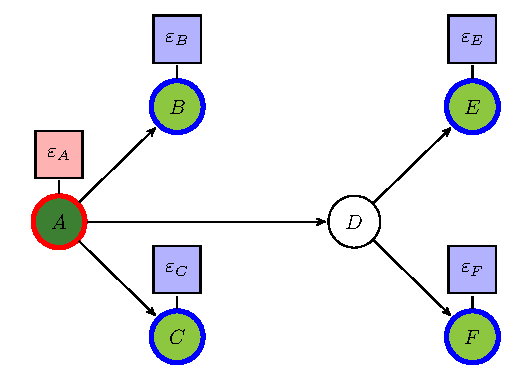
\includegraphics[scale=1.1]{simple-tree/evidence-decomposition-i}}
\hspace*{1cm}
\frame{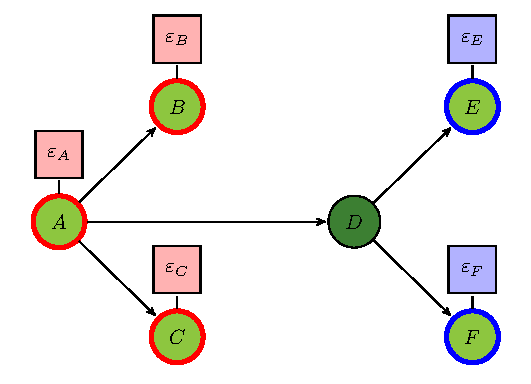
\includegraphics[scale=1.1]{simple-tree/evidence-decomposition-ii}}}

\begin{triangles}
\item Evidence decomposes into up- and downstream evidence
\item Downstream $\EVNEG(V)$ is reachable through child nodes.
\item Upstream $\EVPOS(V)$ is reachable through the predessesor node.
\item Different nodes have totally different decompositions.
\end{triangles}


\foilhead[-1cm]{Initialisation}
\enlargethispage{1cm}
\illustration[scale=0.9]{simple-tree/initialisation}
\vspace*{-0.5cm}
\textbf{Goal.} Assign prior to the root node and likelihood to the leaf nodes.
\begin{align*}
\pi_A(a)&=\pr{A=a|\EVPOS(A)}=\pr{A=a|\textcolor{red}{\varepsilon_A}}\\
\lambda_B(b)&=\pr{\EVNEG(B)|F=f}=\pr{\textcolor{blue}{\varepsilon_B}|B=b}\\
\ldots\\
\lambda_F(f)&=\pr{\EVNEG(F)|F=f}=\pr{\textcolor{blue}{\varepsilon_F}|F=f}
\end{align*}\vspace*{-4ex}\



\foilhead[-1cm]{Likelihood propagation}

\illustration[scale=0.9]{simple-tree/likelihood-propagation-i}

\vspace*{-1.0cm}
\textbf{Inference goal}
\begin{align*}
\lambda_D(d)=\pr{\EVNEG(D)|D=d}
\end{align*}
\textbf{Iterative propagation rules}
\begin{triangles}
\item Independence gives a pooling rule $\lambda_D=\lambda_1\otimes\lambda_2$
\item Marginalisation gives rules $\lambda_1= M_{D\to E}\lambda_E$ and $\lambda_2= M_{D\to F}\lambda_F$.
\end{triangles}


\foilhead[-1cm]{Posterior propagation}
\illustration[scale=0.9]{simple-tree/posterior-propagation-i}
\vspace*{-0.5cm}

\textbf{Inference goal}
\begin{align*}
p_A(a)&=\pr{A=a|\EVPOS(A),\EVNEG(A)}
\end{align*}
\textbf{Iterative propagation rule}
\begin{triangles}
\item Marginal conditional probability $p_A\propto \pi_A\otimes\lambda_A$\vspace*{-1ex}
\end{triangles}


\foilhead[-1cm]{Prior propagation}
\enlargethispage{1cm}
\illustration[scale=0.9]{simple-tree/prior-propagation-i}
\vspace*{-1.5cm}
\textbf{Inference goal}
\begin{align*}
\pi_D(d)&=\pr{D=d|\EVPOS(D)}\\
&=\pr{D=d|\EVPOS(A),\EVNEG(B),\EVNEG(C)}
\end{align*}\vspace*{-4ex}


\textbf{Iterative propagation rule}
\begin{triangles}
\item Prior can be computed as $\pi_D\propto \pi_AM_{A\to D} \otimes M_{A\to B}\lambda_B\otimes M_{A\to C}\lambda_C$\enspace.
\end{triangles}

\middlefoil{Posterior Maximisation}

\foilhead[-1cm]{Posterior maximisation in a simple chain}
\illustration[scale=1.3]{chain-max-i}

\textbf{Inference goal.}
Given evidence at the ends of the chain find the sequence of states $\vec{x}$ that maximise the posterior probability $\pr{\vec{x}|\mathsf{evidence}}$.
\begin{triangles}
\item The log-posterior $\log\pr{\vec{x}|\mathsf{evidence}}$ decomposes into a sum.
\item We must find a sequence with maximal weight.
\item The task can be split into subtask as all subpaths of the path with maximal weight must have maximal weight. 
\item The corresponding iterative algorithm is known as Viterbi algorithm.
\end{triangles}

\foilhead[-1cm]{Posterior maximisation in a simple tree}
\illustration[scale=1.3]{tree-max-i}

\textbf{Inference goal.}
Given evidence at the ends of the chain find the sequence of states $\vec{x}$ that maximise the posterior probability $\pr{\vec{x}|\mathsf{evidence}}$.
\begin{triangles}
\item The log-posterior $\log\pr{\vec{x}|\mathsf{evidence}}$ decomposes into a sum.
\item We must find a tree with maximal weight.
\end{triangles}

\foilhead[-1cm]{Decomposition into subtasks}

\illustration[scale=1.3]{tree-max-i}

All subtrees of the tree with maximal weight must have maximal weight. 
\begin{triangles}
\item We can build chains with maximum weight form leafs
\item We can merge subtrees with maximum weight to maximise the weight.
\item The algorithm works from leafs to the root node.
\item The corresponding iterative algorithm is known as Viterbi algorithm.
\end{triangles}

\middlefoil{Applications}

\foilhead[-1cm]{Rainfall data}

\illustration[scale=0.8]{rainfall_data}
There are two monsoon seasons in Singapore: dry and wet phase.

\foilhead[-1cm]{Modelling with Hidden Markov Model}
\enlargethispage{1cm}
\illustration[scale=0.8]{hidden-markov-model}
Markov chain with states $\SSS=\set{0,1}$ and parameters
\begin{align*}
\vec{\beta}&=(0.5, 0.5)\\
\vec{\alpha}&=
\begin{pmatrix}
0.95 & 0.05\\
0.05 & 0.95\\
\end{pmatrix}
\end{align*}
Emission distributions
\begin{align*}
Y_i|X_i=0\sim\NNN(\mu_0,\sigma_0)\\
Y_i|X_i=1\sim\NNN(\mu_1,\sigma_1)\\
\end{align*}

\foilhead[-1cm]{Belief propagation. Initialisation}

\illustration[scale=1.2]{belief-propagation-in-hmm-i}
\begin{triangles}
\item We have a direct evidence $Y_i=y_i$ for each node $Y_i$. 
\item The likelihood vector is infinite and captured by $\lambda_{Y_i}=\delta_{y_i}$.
\item The local likelihood $\lambda_i^*(x_i)=\pr{Y_i=y_i|x_i}$ is a finite vector. 
\end{triangles}


\foilhead[-1.5cm]{Prior propagation. Filtering}
\enlargethispage{1cm}

\illustration[scale=1.2]{belief-propagation-in-hmm-ii}
\vspace*{-1.0cm}

Prior propagation rule yields
\begin{align*}
\pi_{X_i}(x_i)\propto \sum_{x_{i-1}\in \SSS} \alpha[x_{i-1}, x_i]\cdot\lambda_{i-1}^*(x_{i-1})\cdot \pi_{X_{i-1}}(x_{i-1})
\end{align*}
Now we can do filtering 
\begin{align*}
\pr{x_i|y_1,\ldots,y_{i}}\propto \pi_{X_i}(x_i)\cdot\lambda_i^*(x_i)
\end{align*}

\foilhead[-1.5cm]{Likelihood propagation. Smoothing}
\enlargethispage{1cm}

\illustration[scale=1.2]{belief-propagation-in-hmm-iii}
\vspace*{-1.0cm}

Likelihood propagation rule yields
\begin{align*}
\lambda_{X_i}(x_i)\propto \sum_{x_{i+1}\in \SSS} \alpha[x_{i}, x_{i+1}]\cdot\lambda_{X_{i+1}}(x_{i+1})\cdot \lambda_{i}^*(x_{i})
\end{align*}
Now we can do smoothing 
\begin{align*}
\pr{x_i|y_1,\ldots,y_{n}}\propto \pi_{X_i}(x_i)\cdot\lambda_{X_i}(x_i)
\end{align*}


\foilhead[-1cm]{Annotated rainfall data}

\illustration[scale=0.8]{rainfall_data_with_annotations}

\foilhead[-1cm]{Sensor fusion problem. Kalman filter}

Several sensors measure a physical system
\begin{triangles}
\item Measurements are observable as $\vec{y}\in\RR^p$.
\item Physical system has an hidden state $\vec{x}\in\RR^n$.
\item Physical system evolves linearly $\vec{x}_{i+1}=A\vec{x}_i+\vec{w}_i$.
\item Measurements are linear from the state $\vec{y}_{i}=C\vec{x}_i+\vec{v}_i$.
\end{triangles}
\vspace*{1cm}

Unknown quantities in the system
\begin{triangles}
\item Measurement noise $\vec{v}_t$ is modelled with a normal distribution.
\item Unknown control signal $\vec{w}_i$ is modelled with a normal distribution.
\item Unknown initial state $\vec{x}_0$ is modelled with a normal distribution.
\item Quantities $\vec{x}_0, \vec{v}_i, \vec{w}_i$ are assumed to be independent.
\item All normal distributions can have complex correlation structure.
\end{triangles}

\foilhead[-1cm]{Belief propagation. Initialisation}

\illustration[scale=1.2]{belief-propagation-in-hmm-i}
\begin{triangles}
\item We have a direct evidence $Y_i=y_i$ for each node $Y_i$. 
\item The likelihood vector is infinite and captured by $\lambda_{Y_i}=\delta_{y_i}$.
\item The local likelihood $\lambda_i^*(x_i)=p[Y_i=y_i|x_i]$ is an infinite vector. 
\item The form $\vec{y}_{i}=C\vec{x}_i+\vec{v}_i$ assures that $\vec{y}_{i}|\vec{x}_i$ is normal distribution.
\item The local likelihood $\lambda_i^*$ has a finite description.
\end{triangles}


\foilhead[-1.5cm]{Prior propagation. Filtering}
\enlargethispage{1cm}

\illustration[scale=1.2]{belief-propagation-in-hmm-ii}
\vspace*{-1.0cm}

Prior propagation rule
\begin{align*}
\pi_{X_i}(\vec{x}_i)\propto \int\limits_{\vec{x}_{i-1}} \alpha[\vec{x}_{i-1}, \vec{x}_i]\cdot\lambda_{i-1}^*(\vec{x}_{i-1})\cdot \pi_{X_{i-1}}(\vec{x}_{i-1})d\vec{x}_{i-1}
\end{align*}
leads to a finite description because on the right is a normal distribution. 


\foilhead[-1.5cm]{Likelihood propagation. Smoothing}
\enlargethispage{1cm}

\illustration[scale=1.2]{belief-propagation-in-hmm-iii}
\vspace*{-1.0cm}

Likelihood propagation rule
\begin{align*}
\lambda_{X_i}(x_i)\propto \int\limits_{\vec{x}_{i+1}} \alpha[\vec{x}_{i}, \vec{x}_{i+1}]\cdot\lambda_{X_{i+1}}(\vec{x}_{i+1})\cdot \lambda_{i}^*(\vec{x}_{i}) d\vec{x}_{i+1}
\end{align*}
leads to a finite description because on the right is a normal distribution. 




\end{document}

\foilhead[-1cm]{Reduction to the previous building blocks}

The problem simplifies when we know the vector of hidden states $\vec{x}$: 
\begin{triangles}
\item Inference of emission probabilities $\delta[\ldots]$ reduce to dice throwing.
\item Inference of the chain parameters $\alpha[\ldots]$ and $\beta[\ldots]$ is also possible.
\end{triangles}
\vspace*{2ex}

We can use Viterbi algorithm for finding the most probable hidden state $\vec{x}$ is easy if all parameters are known.
\vspace*{2ex}


\textbf{Naive inference algorithm:} Fix random parameters and repeat steps:
\begin{triangles}
\item Given parameters $\alpha, \beta, \delta$  learn the most probable hidden state $\vec{x}$.
\item Given the most probable hidden state $\vec{x}$ learn model parameters $\alpha, \beta, \delta$.
\end{triangles}
\vspace*{2ex}
This algorithm overfits as all hidden states can have similar probability. 


\foilhead[-0cm]{Model behind naive Bayes classifier}

%\illustration[scale=0.8]{naive-bayes-scheme}

Underlying class value determines observed attributes 
\begin{triangles}
\item Each attribute $X_i$ is binary 
\item All variables are independent if class is fixed
\item Sometimes we just ignore dependancies for easier modelling
\end{triangles}

\foilhead[-0cm]{Likelihood of the data}

Let us assume that we know the probabilities
\begin{align*}
p_i&=\pr{X_i=1|Class=0}\\
q_i&=\pr{X_i=1|Class=1}
\end{align*}
Then using the independence assumption we get
\begin{align*}
\pr{X_1=a_1,\ldots,X_n=a_n|Class=0}&=\prod_{i=1}^np_i^{a_i}(1-p_i)^{1-a_i}\\
\pr{X_1=a_1,\ldots,X_n=a_n|Class=1}&=\prod_{i=1}^nq_i^{a_i}(1-q_i)^{1-a_i}
\end{align*}

\foilhead[-1cm]{Prior and posterior for the class labels}

\enlargethispage{1.5cm}
Now it is straightforward to derive
\begin{align*}
\pr{Class=0|\vec{X}=\vec{a}}&= \frac{\prod\limits_{i=1}^np_i^{a_i}(1-p_i)^{1-a_i}\cdot\pr{Class=0}}{\pr{\vec{X}=\vec{a}}}\\
\pr{Class=1|\vec{X}=\vec{a}}&= \frac{\prod\limits_{i=1}^nq_i^{a_i}(1-q_i)^{1-a_i}\cdot\pr{Class=1}}{\pr{\vec{X}=\vec{a}}}
\end{align*}
which gives an \emph{odd ratio} 
\begin{align*}
\frac{\pr{Class=0|\vec{X}=\vec{a}}}{\pr{Class=1|\vec{X}=\vec{a}}}&=\frac{\pr{Class=0}}{\pr{Class=1}}\cdot\frac{\prod\limits_{i=1}^np_i^{a_i}(1-p_i)^{1-a_i}}{\prod\limits_{i=1}^nq_i^{a_i}(1-q_i)^{1-a_i}}
\end{align*} 
 
\foilhead[-1cm]{The resulting classifier is a linear classifer}
 
By taking logarithm form the odd ratio we get
\begin{align*}
\log\left(\frac{\pr{Class=0|\vec{X}=\vec{a}}}{\pr{Class=1|\vec{X}=\vec{a}}}\right)&= w_0+\sum_{i=1}^n w_ia_i
\end{align*} 
where 
\begin{align*}
w_0&=\log\left(\frac{\pr{Class=0}}{\pr{Class=1}}\right)+\sum_{i=1}^n\log\left(\frac{1-p_i}{1-q_i}\right)\\
w_i&=\log \left(\frac{p_i}{1-p_i}\cdot\frac{1-q_i}{q_i}\right) 
\end{align*}

\foilhead[-1cm]{How to train the classifier?}
A frequentistic approach is to fix probabilities from the training sample
\begin{align*}
p_i&=\frac{\#\set{\text{data points form class 0 with $X_i=1$}}}{\#\set{\text{data points form class 0}}}\\
q_i&=\frac{\#\set{\text{data points form class 1 with $X_i=1$}}}{\#\set{\text{data points form class 1}}}
\end{align*}
However if some value does not occur for $X_i$ in the training sample we get overly confident results. Thus, Bayesian mean estimate is better alternative  
\begin{align*}
p_i&=\frac{\#\set{\text{data points form class 0 with $X_i=1$}}+1}{\#\set{\text{data points form class 0}}+2}\\
q_i&=\frac{\#\set{\text{data points form class 1 with $X_i=1$}}+1}{\#\set{\text{data points form class 1}}+2}
\end{align*}

\end{document}

\foilhead[-1cm]{Going beyond naive Bayesian models}
\illustration[scale=0.8]{bayesian-network}

Complex causal models are often defined through Bayesian networks
\begin{triangles}
\item A complex processes is first split into sub-events
\item Direct causal dependencies between sub-events are detected
\item Causation mechanisms are characterised with probability tables
\end{triangles} 
  
\foilhead[-1cm]{Strength and weaknesses of Bayesian networks}

\textbf{Strengths}
\begin{triangles}
\item Bayesian networks are easy to interpret
\item Bayesian networks are good for formalising fuzzy background knowledge
\item Estimation of individual probability tables is tractable
\item There are tools for doing inference with Bayesian networks  
\end{triangles}
\vspace*{1cm}

\textbf{Weaknesses}
\begin{triangles}
\item You must know the causal structure of sub-events  
\item Identification of causal structure form data alone is very difficult
\item It is notoriously difficult to model non-trivial causal dependencies
\item Standard inference procedures often do not have closed solutions 
\end{triangles}

\end{document}
